\documentclass[12pt, twoside]{article}
\usepackage[letterpaper, margin=1in, headsep=0.5in]{geometry}
\usepackage[english]{babel}
\usepackage[utf8]{inputenc}
\usepackage{amsmath}
\usepackage{amsfonts}
\usepackage{amssymb}
\usepackage{tikz}
\usetikzlibrary{quotes, angles}
\usepackage{graphicx}
\usepackage{enumitem}
\usepackage{multicol}

\newif\ifmeta
\metatrue %print standards and topics tags

\title{IB Mathematics}
\author{Chris Huson}
\date{September 2021}

\usepackage{fancyhdr}
\pagestyle{fancy}
\fancyhf{}
\renewcommand{\headrulewidth}{0pt} % disable the underline of the header
\raggedbottom


\fancyhead[LE]{\thepage}
\fancyhead[RO]{\thepage \\ Name: \hspace{4cm} \,\\}
\fancyhead[LO]{BECA / IB Math 01-Linear functions\\* 17 September 2021}

\begin{document}

\subsubsection*{1.4 Homework: Functions}
\begin{enumerate}
\item The graph of a function $f$ is shown on the grid below.
\begin{multicols}{2}
\begin{enumerate}
  \item Write down $f(-1)$
  %\vspace{0.25cm}
  \item Find $x$ for $f(x)=5$.
  \vspace{0.25cm}
  \item Label which is the domain and which is the range.
  \begin{enumerate}
    \item $(0,5]$
    \item $-2<x \leq 3$
  \end{enumerate}
\end{enumerate}
  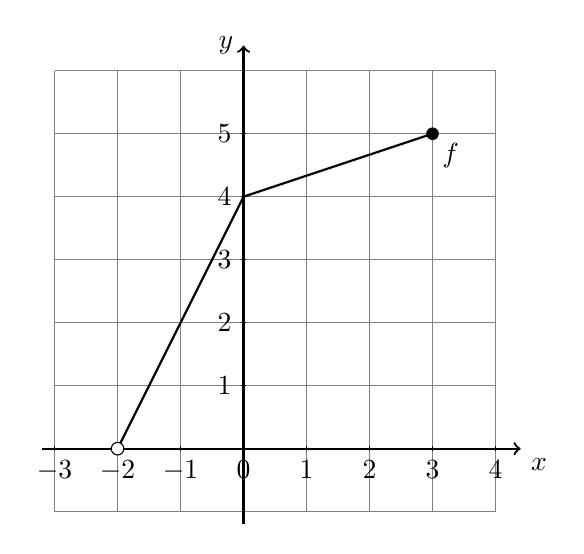
\begin{tikzpicture}[scale=0.8]
    \draw [help lines] (-3,-1) grid (4,6);
    \draw [thick, ->] (-3.2,0) -- (4.4,0) node [below right] {$x$};
    \draw [thick, ->] (0,-1.2)--(0,6.4) node [left] {$y$};
    \foreach \x in {-3, -2, ..., 4} \draw (\x cm,1pt) -- (\x cm,-1pt) node[anchor=north] {$\x$};
    \foreach \y in {1, 2, 3, 4, 5} \draw (1pt,\y cm) -- (-1pt,\y cm) node[anchor=east] {$\y$};
    \draw [thick] (-2,0) -- (0,4) -- (3,5);
    \fill (3,5) circle[radius=0.1] node[below right]{$f$};
    \fill [white] (-2,0) circle[radius=0.1];
    \draw (-2,0) circle[radius=0.1];
  \end{tikzpicture}
\end{multicols}

\item A relation composed of four points is plotted on the graph below, and represented as a set of ordered pairs as $\{ (j,2),(1,4),(3,2),(4,k) \}$
\begin{multicols}{2}
\begin{enumerate}
  \item Write down $j$
  \item Write down $k$
  \item Is the relation a function? Why or why not. \vspace{2cm}
  \item Add an ordered pair to the relation so that it would \emph{not} be a function.
\end{enumerate}
  \begin{center} %4 quadrant regents grid w T-Chart
  \begin{tikzpicture}[scale=0.8]
    %\draw [help lines] (-3,-2) grid (4,6);
    \draw [thick, ->] (-3.2,0) -- (5.4,0) node [below right] {$x$};
    \draw [thick, ->] (0,-1.2)--(0,6.4) node [left] {$y$};
    \foreach \x in {-2, -1, ..., 5} \draw (\x cm,1pt) -- (\x cm,-1pt) node[anchor=north] {$\x$};
    \foreach \y in {1, 2, 3, 4, 5} \draw (1pt,\y cm) -- (-1pt,\y cm) node[anchor=east] {$\y$};
    %\draw [thick, <->] (-3.5,-1.5) -- (4.2,6.2);
    \fill (1,4) circle[radius=0.1] node[above right]{$(1,4)$};
    \fill (3,2) circle[radius=0.1] node[above]{$(3,2)$};
    \fill (-2,2) circle[radius=0.1] node[above]{$(j,2)$};
    \fill (4,1) circle[radius=0.1] node[above right]{$(4,k)$};
  \end{tikzpicture}
  \end{center}
\end{multicols}
\vspace{0.25cm}

\item An athlete finds that the number of reps she can lift is a function of the weight. 
\begin{center}
  \begin{tabular}{|l|r|r|r|r|r|r|}
    \hline
    Weight (lbs) & 10 & 15 & 20 & 25 & 30\\ 
    \hline 
    Reps & 18 & 12 & 3 & 0 & 0\\ 
    \hline 
  \end{tabular}
\end{center}
\begin{enumerate}
  \item How many times can she lift 20 pounds?\vspace{0.25cm}
  \item What is the domain of the function shown in the table?\vspace{0.25cm}
  \item Estimate the maximum weight she can lift.
\end{enumerate}

\newpage
\item In the following two problems, solve for the value of $x$.
  \begin{multicols}{2}
    \begin{enumerate}
      \item   $2x-3=12-x$ \vspace{6cm}
      \item   $(3x-2)+(x-6)=0$ \vspace{6cm}
    \end{enumerate}
  \end{multicols}
    \vspace{3cm}

\item Given the linear function $f(x)=5x-7$.
\begin{multicols}{2}
  \begin{enumerate}
    \item Find $f(-1)$ \vspace{6cm}
    \item   $f(x)=8$. Find $x$. \vspace{6cm}
  \end{enumerate}
\end{multicols}
  \vspace{6cm}

\item Two functions $f$ and $g$ are shown on the grid below.
\begin{multicols}{2}
\begin{enumerate}
  \item What is the equation of $f$?
  %\vspace{0.25cm}
  \item What is the equation of $g$?
  \vspace{0.25cm}
  \item What is the intersection of the lines as an ordered pair.
\end{enumerate}
  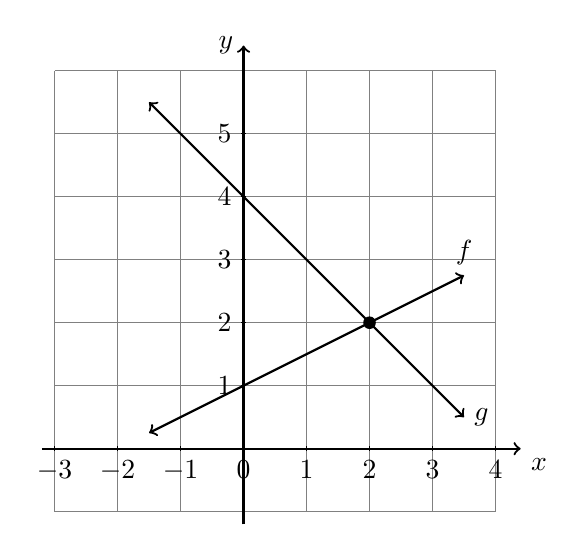
\begin{tikzpicture}[scale=0.8]
    \draw [help lines] (-3,-1) grid (4,6);
    \draw [thick, ->] (-3.2,0) -- (4.4,0) node [below right] {$x$};
    \draw [thick, ->] (0,-1.2)--(0,6.4) node [left] {$y$};
    \foreach \x in {-3, -2, ..., 4} \draw (\x cm,1pt) -- (\x cm,-1pt) node[anchor=north] {$\x$};
    \foreach \y in {1, 2, 3, 4, 5} \draw (1pt,\y cm) -- (-1pt,\y cm) node[anchor=east] {$\y$};
    \draw [thick, <->] (-1.5,0.25) -- (3.5, 2.75) node[above]{$f$};
    \draw [thick, <->] (-1.5,5.5) -- (3.5, 0.5) node[right]{$g$};
    \fill (2,2) circle[radius=0.1];
  \end{tikzpicture}
\end{multicols}

\end{enumerate}
\end{document}